\subsection{Subpaso 1-A: Iniciar sanción para el solicitante}
Una vez buscado el solicitante nos muestra la siguiente interfaz
\begin{figure}[hbtp]

	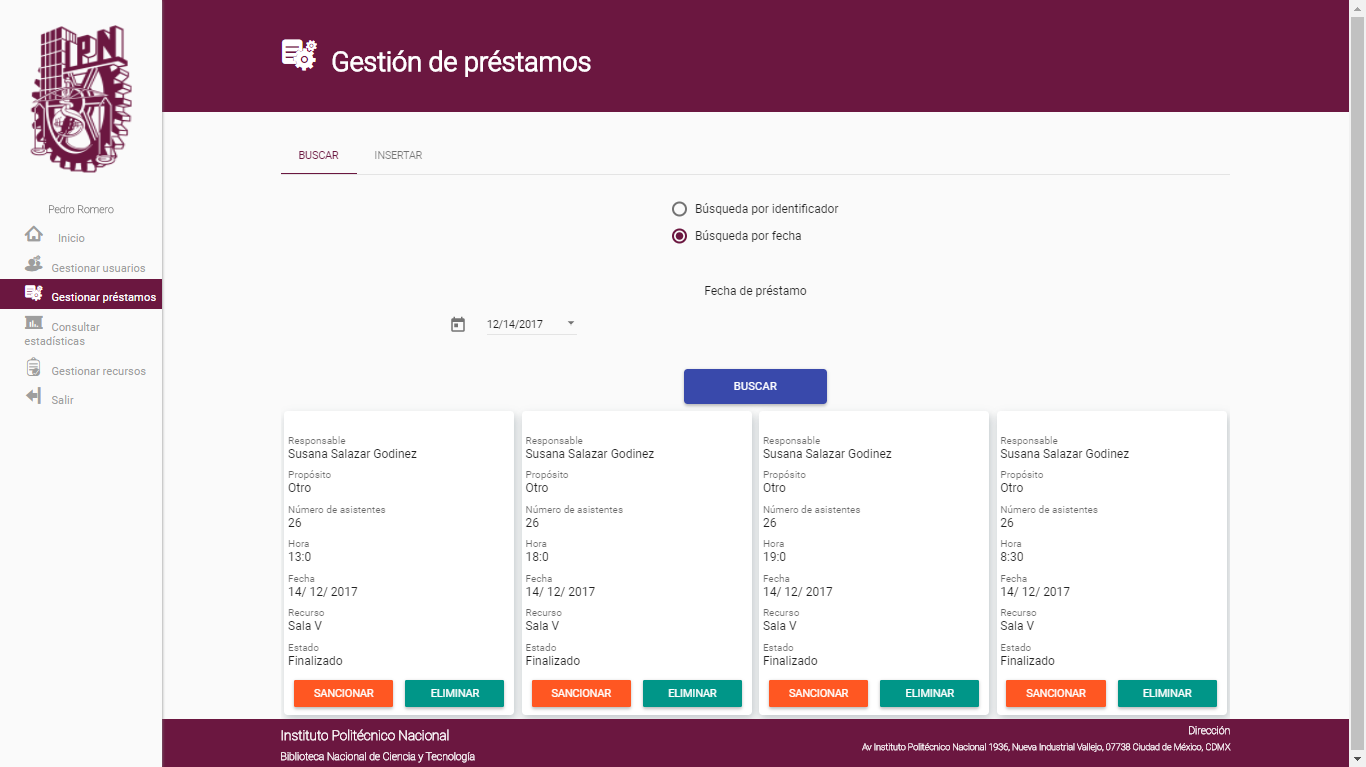
\includegraphics[scale=0.3]{images/Interfaz/IUGS07_busqueda.PNG}
	\caption{Busqueda Solicitante}
	\end{figure}

	Para acceder a sancionar a un solicitante se puede ingresar de tres maneras:
	\begin{enumerate}
		\item presione el botón \textbf{Sancionar} que corresponda 
			al responsable a sancionar, este botón aparece en la parte 
			inferior de la interfaz
		\begin{figure}[hbtp]

	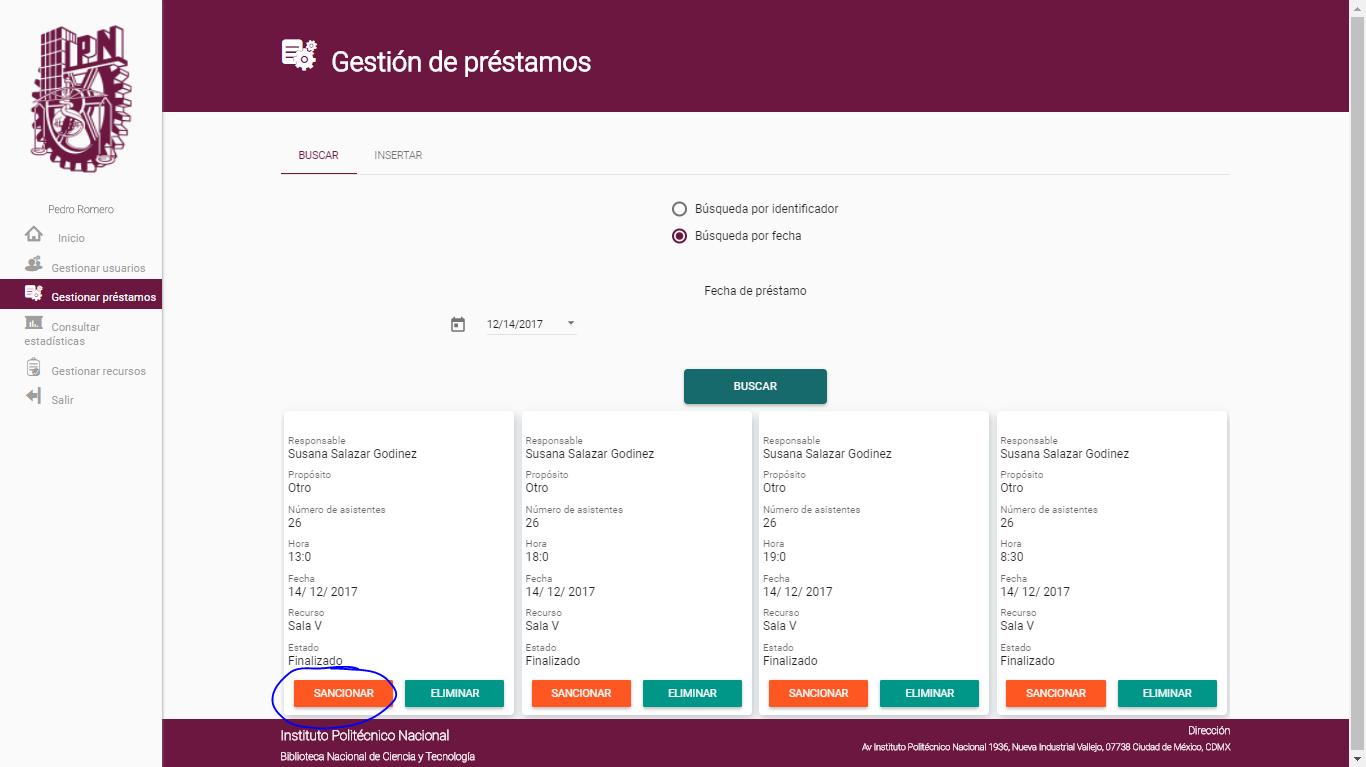
\includegraphics[scale=0.3]{images/Interfaz/IUGS07_sancionarBoton.PNG}
	\caption{Sancionar Solicitante}
	\end{figure}	 
		
	\end{enumerate}

	